\documentclass[10pt,a4paper]{article}
\usepackage[utf8]{inputenc}
\usepackage[english]{babel}
\usepackage{amsmath}
\usepackage{amsfonts}
\usepackage{amssymb}
\usepackage{graphicx}
\usepackage[left=2cm,right=2cm,top=2cm,bottom=2cm]{geometry}
\author{Marco Biroli}
\usepackage{physics}
\usepackage{slashed}
\usepackage{stmaryrd}
\title{Master ENS ICFP - First Year 2020/2021\\
Relativistic Quantum Mechanics and Introduction to Quantum Field Theory\\
Mid Term Homework}

\begin{document}
\maketitle

\section[Exercise]{Some operator identities : 6 points}

\begin{enumerate}

\item Consider $F(t) = e^{tA} B e^{-tA}$ then consider the following inductive hypothesis: 
\[\mathcal{H}_n : " \dv[n]{F(t)}{t} = e^{tA} \underbrace{[A, [A, \cdots, [A, B]\cdots]}_{n \mbox{~commutators}} e^{-tA} "\]
The base case $n= 1$ is trivially satisfied:
\[
\dv{F(t)}{t} = e^{tA} A B e^{-tA} + e^{tA} B (-A) e^{-tA} = e^{tA} (AB - BA) e^{-tA} = e^{tA}[A, B] e^{-tA}
\]
Then suppose $\mathcal{H}_n$ for $n \in \mathbb{N}$. Then we have that:
\begin{align*}
\dv[n+1]{F(t)}{t} &= \dv{}{t} \dv[n]{F(t)}{t} = \dv{}{t} e^{tA} \underbrace{[A, [A, \cdots, [A, B]\cdots]}_{n \mbox{~commutators}} e^{-t A } \\
&= e^{tA} A \underbrace{[A, [A, \cdots, [A, B]\cdots]}_{n \mbox{~commutators}} e^{-tA} + e^{tA} \underbrace{[A, [A, \cdots, [A, B]\cdots]}_{n \mbox{~commutators}} (-A) e^{-tA}\\
&= e^{tA} (A\underbrace{[A, [A, \cdots, [A, B]\cdots]}_{n \mbox{~commutators}} - \underbrace{[A, [A, \cdots, [A, B]\cdots]}_{n \mbox{~commutators}} A) e^{-tA}\\
&= e^{tA} \underbrace{[A, [A, \cdots, [A, B]\cdots]}_{n + 1 \mbox{~commutators}} e^{-tA}
\end{align*}
Hence if $\mathcal{H}_n$ is true for $n \in \mathbb{N}$ so is $\mathcal{H}_{n+1}$ then by induction we can conclude that $\mathcal{H}_n$ is true for all $n \in \mathbb{N}$. Hence we have that:
\[
F(t) = F(0) + \sum_{n = 1}^{+\infty} \frac{t^n}{n!} \dv[n]{F(t)}{t}\Big|_{t = 0} = B + \sum_{n = 1}^{+\infty} \frac{t^n}{n!} \underbrace{[A, [A, \cdots, [A, B]\cdots]}_{n \mbox{~commutators}}
\]
Hence:
\[
e^{A} B e^{-A} = F(1) = B + \sum_{n=1}^{+\infty} \frac{1}{n!} \underbrace{[A, [A, \cdots, [A, B]\cdots]}_{n \mbox{~commutators}}
\]

\item Let $G(t) = e^{tA} e^{tB}$.  Then notice that:
\begin{align*}
\dv{G(t)}{t} &= A e^{tA} e^{t B} + e^{tA} e^{tB} B = A e^{tA} e^{tB} + e^{tA} B e^{-tA} e^{tA} e^{tB} = A e^{tA} e^{t B} + (B + t[A, B] + 0) e^{tA} e^{tB}\\
&= (A + B + t[A, B]) e^{tA} e^{tB} = (A + B + t[A, B]) G(t) 
\end{align*}
Therefore $G$ is a solution to the differential equation:
\[
\partial_t f(t) = (A + B + t[A, B]) f(t)
\]
Now notice furthermore that:
\[
\partial_t e^{tA + tB + \frac{t^2}{2} [A, B]} = (A + B + t[A, B])e^{tA + tB + \frac{t^2}{2}[A, B]}
\]
And identically:
\[
\partial_t e^{\frac{t^2}{2}[A, B]} e^{tA + tB} = t[A, B] e^{\frac{t^2}{2}[A, B]} e^{t A + tB} + e^{\frac{t^2}{2}[A, B]} (A + B) e^{tA + tB} = (A + B + t[A, B])e^{\frac{t^2}{2}[A, B]} e^{tA + tB} 
\]
Hence all three functions are solution to the same differential equation and furthermore at $t = 0$ they are all equal to the identity hence they must be equal for all $t$. Then taking $t = 1$ gives the desired equalities.


\item We have that:
\[
[F, G^\dagger] = [\sum_j f_j a_j, \sum_j g_j^\star a_j^\dagger] = \sum_{j, k = 0}^{+\infty} f_j g_k^\star [a_j, a_k^\dagger] = \sum_{j, k = 0}^{+\infty} f_j g_k^\star \delta_{jk} = \sum_{j = 0}^{+\infty} f_j g_j^\star
\]
Furthermore we have that $[F, G^\dagger] \propto \text{Id}$ and therefore we trivially have that $[F, [F, G^\dagger]] = [G^\dagger, [F, G^\dagger]] = 0$. Now applying question 2 we have that:
\[
e^{G^\dagger} e^F = e^{-\frac{1}{2} \sum_{j} f_j g_j^\star } e^{G^\dagger + F} \Rightarrow  e^{\frac{1}{2} \sum_{j} f_j g_j^\star }e^F =  \underbrace{e^{\frac{1}{2} \sum_{j} f_j g_j^\star } e^{-\frac{1}{2} \sum_{j} f_j g_j^\star }}_{=e^A e^{-A}} e^{G^\dagger + F}
\]
Now from Question 1 we have that for any $A$ (trivially $[A, \text{Id}] = 0$) we get:
\[
e^A \text{Id} e^{-A} = \text{Id} + \sum_{n=1}^{+\infty} \frac{1}{n!} \cdot 0 = \text{Id}
\]
Hence the above formula simplifies to:
\[
e^{F + G^\dagger} = e^{\frac{1}{2}\sum_j f_jg_j^\star} e^{G^\dagger} e^F
\]

\item Similarly as before let $F = \int \dd^3 \vb{q} f(\vb{q}) a(\vb{q})$ and $G = \int \dd^3 \vb{q} h(\vb{q})^\dagger a(\vb{q})$. Then we have that:
\[
[F, G^\dagger] = [ \int \dd^3 \vb{q} f(\vb{q}) a(\vb{q}), \int \dd^3 \vb{q} h(\vb{q}) a^\dagger(\vb{q})] = \int \dd^3 \vb{q} f(\vb{q})h(\vb{q})[a(\vb{q}), a^\dagger(\vb{q})] = \int \dd^3 \vb{q} f(\vb{q}) h(\vb{q})
\]
A similar direct application of 2 gives the desired result.

\end{enumerate}

\section[Exercise]{An example of an asymptotic series}

We have that:
\[
f(g) = \frac{1}{\sqrt{\pi}} \int_{-\infty}^{+\infty} \dd x e^{-x^2 - g x^4} \mbox{~~hence~~} |f(g)| < \int_{-\infty}^{+\infty} \dd x | e^{-x^2 - g x^4}| = \int_{-\infty}^{+\infty} \dd x e^{-x^2 - x^4 \Re g} < \int_{-\infty}^{+\infty} \dd x e^{-x^4 \Re g}
\]
Hence as long as $\Re g > 0$ this is obviously well defined from the last term and if $\Re g = 0$ this is obviously well defined from the before last term.

\begin{enumerate}
\item This integral admits an exact solution given by:
\[
f(g) = \frac{e^{\frac{1}{8g}} K_{\frac{1}{4}}(\frac{1}{8g})}{2\sqrt{\pi g}} \delta_{\Re g > 0} + \delta_{\Re g = 0} \mbox{~~where~~} K_n(z) \mbox{~~is the modified Bessel function of the second kind.}
\]
The plot of the numerical values for $g \in [0.01, 1]$ is given in Figure \ref{integral:1}.
\begin{figure}
\centering
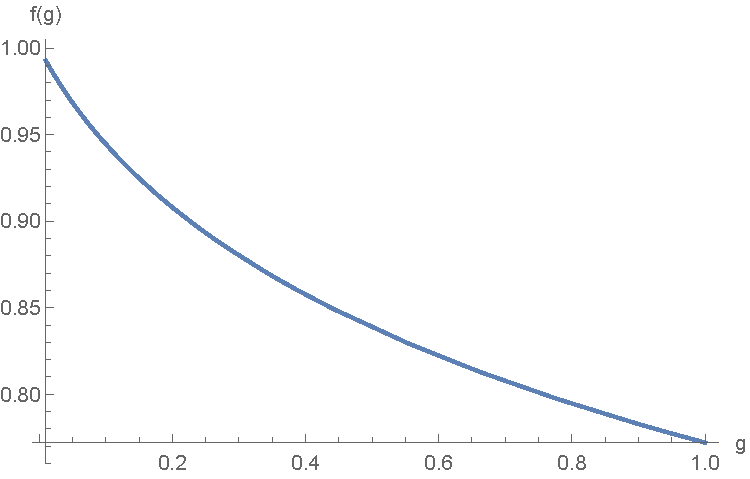
\includegraphics[width = 0.5\textwidth]{integral1}
\caption{Plot of the numerical values of $f(g)$ for $g \in [0.01, 1]$. }\label{integral:1}
\end{figure}
Then $f(g)$ decreases monotonically when $g > 0$ increases since:
\[
\dv{}{g} f(g) = \frac{1}{\sqrt{\pi}} \int_{-\infty}^{+\infty} \dd x (-x^4) e^{-x^2 - g x^4} = \frac{-1}{\sqrt{\pi}} \underbrace{\int_{-\infty}^{+\infty} x^4 e^{-x^2 - g x^4}}_{ > 0 \mbox{~~when~~} g \in \mathbb{R}^+} < 0
\]

\item We have that:
\[
e^{-g x^4} = \sum_{n = 0}^{+\infty} \frac{(-gx^4)^n}{n!}
\]
And plugging this in the expression of $f$ and inverting the sum and the integral gives:
\[
\frac{1}{\sqrt{\pi}} \sum_{n = 0}^{+\infty} \frac{(-g)^n}{n!} \int_{-\infty}^{+\infty} \dd x\,\, x^{4n} e^{-x^2}
\]
We notice the integral ressembles strongly the gamma function hence we change variables by taking $u = x^2$ ($\dd u = 2 \sqrt{u} \dd x$) and we get:
\[
2^{-1} \int_{-\infty}^{+\infty} \dd u u^{2n - \frac{1}{2}} e^{-u} = 2^{-1} \Gamma(2n + \frac{1}{2}) = 2^{-4n} \sqrt{\pi} \frac{\Gamma(4n)}{\Gamma(2n)} \mbox{~~from the Legendre duplication formula.}
\]
Hence plugging it back up top we obtain:
\[
\tilde{f}(g) = \sum_{n = 0}^{+\infty} \left( \frac{(-1)^n(4n)!}{n! 2^{4n} (2n)!} \right) g^n
\]
Notice that the terms $f_n$ are monotonically increasing in norm and diverge hence the sum does not converge absolutely and $R = 0$ and it also does not converge conditionally. 

\item \begin{figure}
\centering
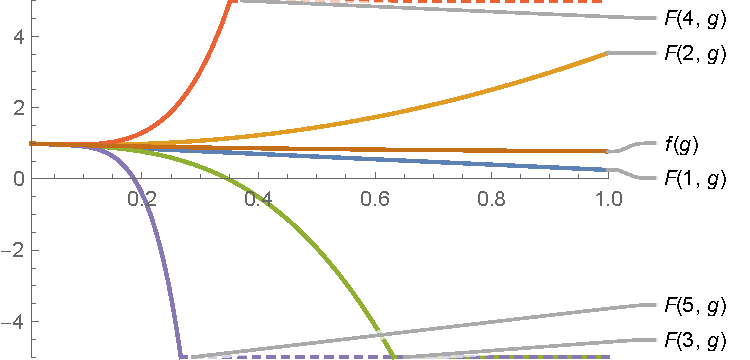
\includegraphics[width=0.44 \textwidth]{approx_series}
\hspace{0.1\textwidth}
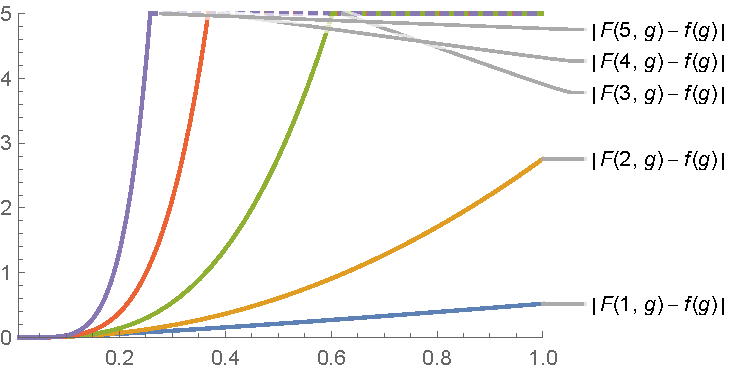
\includegraphics[width=0.44 \textwidth]{error_series}
\caption{Series approximations of $f(g)$ and their errors for $g \in [0.01, 1]$.}
\end{figure}

We can see that the speed of the divergence is very strongly related to the value of $g$ if $g \ll 1$ the divergence is negligible but as soon as $g \sim 1$ the divergence is clearly apparent. 

\end{enumerate}


\section{A relation between Dirac spinors}

\begin{enumerate}

\item Remember that up to a re-writing we have that:
\[
\omega_{ij} = \varepsilon_{i j k} \theta^k \mbox{~~and~~} \omega^{k0} = \nu^k \mbox{~~and~~} \omega_{\mu \nu} = 0 \mbox{~~otherwise.}
\]
Where the $\theta^k$ represent the rotations in the 3 spatial dimensions and the $\nu^k$ represent the boosts along the the three spatial directions. Hence the representation of $L(\vb{p})$ trivially has that $\theta^k = 0$. Then we have that:
\[
i \gamma^0 D(L(\vb{p})) i \gamma^0 = i \gamma^0 \exp( \frac{1}{4} \omega_{\mu \nu} (\gamma^\mu \gamma^\nu - \gamma^\nu \gamma^\mu) ) i \gamma^0
\] 
Now in order to simplify we need to bring the product with the gamma matrices inside. To do so we need to remember two properties. Firstly we have that $(i\gamma^0) = (i\gamma^0)^{-1}$ and secondly we have that: $P e^A P^{-1} = e^{P A P^{-1}}$. Hence applying this formula here we obtain that:
\[
i\gamma^0 D(L(\vb{p})) i \gamma^0 = \exp(\frac{\omega_{\mu \nu}}{4} i\gamma^0 (\gamma^\mu \gamma^\nu - \gamma^\nu \gamma^\mu) i\gamma^0   ) = \exp(\frac{\omega_{\mu \nu}}{4} (i \gamma^0 \gamma^\mu i \gamma^0 i \gamma^0 \gamma^\nu i \gamma^0 - i\gamma^0\gamma^\nu \i \gamma^ 0 i \gamma^0 \gamma^\mu i\gamma^0)   )
\] 
Now we use the formula from the course: $i\gamma^0 \gamma^\mu i \gamma^0 = P^\mu_\nu \gamma^\nu$ where $P^\mu_\nu$ is the parity operator defined in (3.33). Hence this means that the terms in the exponential simplify to:
\[
i\gamma^0 D(L(\vb{p})) i \gamma^0 = \exp(\frac{\omega_{\mu \nu}}{4}  (\gamma^\mu \gamma^\nu - \gamma^\nu \gamma^\mu) (-1)^{1 - \delta^\mu_0}  (-1)^{1 - \delta^\nu_0}) = \exp(\frac{\omega_{\mu \nu}(-1)^{\delta^\mu_0 + \delta^\nu_0 - \delta^\mu_0 \delta^\nu_0} }{4}  (\gamma^\mu \gamma^\nu - \gamma^\nu \gamma^\mu)) 
\]
Hence now we take $\omega'_{\mu \nu} = \omega_{\mu \nu}(-1)^{\delta^\mu_0 + \delta^\nu_0 - \delta^\mu_0 \delta^\nu_0}$, now since $\omega_{00} = 0$ we can discard the term $\delta^\mu_0 \delta^\nu_0$ which means that we are left with:
\[
\omega'_{\mu \nu } = \omega_{\mu \nu}(-1)^{\delta^\mu_0 + \delta^\nu_0} \Leftrightarrow \omega'_{ij} = \omega_{ij} \land \omega'_{k 0} = - \omega_{k 0} \Rightarrow \theta'^k = \theta^k \land \nu'^k = -\nu^k
\]
Hence we have that:
\[
i\gamma^0 D(L(\vb{p})) i \gamma^0 = D(L(-\vb{p}))
\]

\item We have that:
\[
(i p_\mu \gamma^\mu + m) u(\vb{p}, \sigma) = 0 \mbox{~~and~~} (-i p_\mu \gamma^\mu + m) v(\vb{p}, \sigma) = 0
\]
Hence if we take $\vb{p} = 0$ and $p_0 = -p^0 = -m$ for a particle at rest the above simplifies to:
\[
(-im \gamma^0 + m) u(\vb{0}, \sigma) = 0 \mbox{~~and~~} (i m \gamma^0 + m) v(\vb{0}, \sigma) = 0
\]
Which up to dividing by $m$ simplifies to:
\[
(-i \gamma^0 + \vb{1}) u(\vb{0}, \sigma) = 0 \mbox{~~and~~} (i\gamma^0 + \vb{1}) v(\vb{0}, \sigma) = 0
\]
Hence up to a re-writing we have that:
\[
i\gamma^0 u(\vb{0}, \sigma) = u(\vb{0}, \sigma) \mbox{~~and~~} i\gamma^0 v(\vb{0}, \sigma) = - v(\vb{0}, \sigma)
\]
Then from the definition of $u, v$ and $D(L(\vb{p}))$ we have that $u(\vb{p}, \sigma) = D(L(\vb{p})) u(\vb{0}, \sigma)$ and identically for $v$. Hence we have that:
\[
i \gamma^0 u(\vb{p}, \sigma) = i \gamma^0 D(L(\vb{p})) u(\vb{0}, \sigma) = i \gamma^0 D(L(\vb{p})) i \gamma^0 i \gamma^0 u(\vb{0}, \sigma) = D(L(-\vb{p})) u(\vb{0}, \sigma) = u(-\vb{p}, \sigma)
\]
And identically:
\[
i\gamma^0 v(\vb{p}, \sigma) = i\gamma^0 D(L(\vb{p})) v(\vb{0}, \sigma) = i \gamma^0 D(L(\vb{p})) i \gamma^0 i \gamma^0 v(\vb{0}, \sigma) = D(L(-\vb{p})) (-v(\vb{0}, \sigma)) = - v(-\vb{p}, \sigma) 
\]

\end{enumerate}


\section{Some traces of products of $\gamma$-matrices}

We have that:
\[
\tr \gamma_\mu \gamma_\nu = \tr {\gamma_\mu, \gamma_\nu} - \gamma_\nu \gamma_\mu = 2 \tr \eta_{\mu \nu} I_4 - \tr \gamma_\nu \gamma_\mu = 2 \tr \eta_{\mu \nu} I_4 - \tr \gamma_\mu \gamma_\nu
\]
Hence adding on both side we obtain the desired equality:
\[
\tr \gamma_\mu \gamma_\nu = \eta_{\mu \nu} \tr I_4 = 4 \eta_{\mu \nu}
\]
Similarly we have that:
\[
\tr \gamma_\mu \gamma_\nu \gamma_\rho \gamma_\sigma = \tr \gamma_\mu \gamma_\nu (2\eta_{\rho \sigma} I_4 - \gamma_\sigma \gamma_\rho) = 2\eta_{\rho \sigma} \tr \gamma_\mu \gamma_\nu - \tr \gamma_\mu \gamma_\nu \gamma_\sigma \gamma_\rho = 2 \eta_{\rho \sigma} 4 \eta_{\mu \nu} - \tr \gamma_\mu \gamma_\nu \gamma_\sigma \gamma_\rho 
\]
Now we can repeat the argument but instead of permuting the last two term we permute the two middle terms and then we permute the first two terms in such a way as to bring $\gamma_\sigma$ to the front of the queue. Then we have that:
\[
\tr \gamma_\mu \gamma_\nu \gamma_\rho \gamma_\sigma = 2 \eta_{\rho \sigma} 4 \eta_{\mu \nu} -  2 \eta_{\nu \sigma} 4 \eta_{\mu \rho} + 2 \eta_{\mu \sigma} 4 \eta_{\nu \rho} - \tr \gamma_\sigma \gamma_\mu \gamma_\nu \gamma_\rho
\]
Then from the cyclicity of the trace we can bring $\gamma_\sigma$ to the back again. Hence we obtain:
\[
\tr \gamma_\mu \gamma_\nu \gamma_\rho \gamma_\sigma = 4(\eta_{\rho \sigma} \eta_{\mu \nu} + \eta_{\nu \sigma} \eta_{\mu \rho} - \eta_{\mu \sigma} \eta_{\nu \rho})
\]
Now for the last trace property of the $\gamma$-matrices. We have that:
\[
\tr \gamma_{\mu_1} \cdots \gamma_{\mu_{2n+1}} = \tr \gamma_5 \gamma_5 \gamma_{\mu_1} \cdots \gamma_{\mu_{2n+1}} = (-1)^{2n+1}\tr \gamma_5 \gamma_{\mu_1}\cdots \gamma_{\mu_{2n + 1}} \gamma_5 = - \tr \gamma_{\mu_1} \cdots \gamma_{\mu_{2n + 1}}
\]
Where in the first equality we used that $\gamma_5^2 = 1$ and in the second that $\gamma_5 \gamma_\mu = - \gamma_\mu \gamma_5$. From the above we can then conclude that:
\[
\tr \gamma_{\mu_1} \cdots \gamma_{\mu_{2n+1}} = 0
\]

\section{Energy levels of a relativistic charged spin-0 particle in a harmonic electrostatic potential}

\begin{enumerate}


\item From these relation we have that:
\begin{align*}
X^2 \ket{n} &= \frac{1}{2 m \Omega} \left( a^2 + (a^\dagger)^2 + \{a, a^\dagger\} \right)\ket{n} \\
&= \frac{1}{2m \Omega} (\sqrt{n}\sqrt{n-1} \ket{n-2} + \sqrt{n+1}\sqrt{n+2} \ket{n+2} + (n+1)\ket{n} + n\ket{n})
\end{align*}
Hence we get that:
\[
\bra{n} X^4 \ket{n} = (\bra{n} X^2)(X^2 \ket{n}) = \frac{6}{(2 m \Omega)^2} \left( n(n + 1) + \frac{1}{2} \right) 
\]

\item We have that:
\[
(-D_\mu D^\mu + m^2) \Phi = 0 \mbox{~~where~~} D^\mu = \partial^\mu - i q A^\mu
\]
Expanding this slightly gives:
\[
\left((\partial_t + i \frac{m}{2} \omega^2 x^2)^2 - \laplacian + m^2\right)\Phi = 0
\]
Now inserting the Ansatz we are given: $\Phi = e^{-iEt} \phi$ this gives:
\[
(\partial_t + i \frac{m}{2} \omega^2 x^2)^2 e^{-iE t} \phi +   e^{-iEt} (-\laplacian + m^2) \phi = 0
\]
Hence to simplify we compute:
\[
e^{iEt}(\partial_t + i \frac{m}{2} \omega^2 x^2)^2 e^{-iEt} = e^{iEt}(\partial_t^2 + i m \omega^2 x^2 \partial_t - \frac{m^2}{4} \omega^4 x^4) e^{-i E t} = - E^2 + m \omega^2 x^2 E - \frac{m^2}{4} \omega^4 x^4
\]
Putting everything together we obtain:
\[
\left( E^2 - m\omega^2 x^2 E + \frac{m^2}{4} \omega^4 x^4 + \laplacian - m^2 \right) \phi = 0
\]

\item We see from the above that the coefficients depend only on $x$ hence the equation is invariant for translations in $y$ and $z$. We therefore know that the solution can be written as:
\[
\phi(x, y, z) = e^{i k_y y} e^{i k_z z} f(x) 
\]
Plugging this in the equation on top we obtain:
\[
\left( E^2 - m \omega^2 x^2 E + \frac{m^2}{4} \omega^4 x^4 - k_y^2 - k_z^2 + \partial_x^2 - m^2 \right) f(x) = 0
\]
Hence reorganizing the terms we obtain:
\[
\left(-\frac{\partial_x^2}{2m} + \underbrace{\frac{\omega^2 E}{2}}_{\alpha} x^2 - \underbrace{\frac{m}{8} \omega^4}_{\beta} x^4 \right)f = \underbrace{\frac{1}{2m}\left(E^2 - k_y^2 - k_z^2 - m^2\right)}_{\varepsilon} f 
\]
Now if we consider the $x^4$ term as a perturbation the base energies are the ones of the harmonic oscillator which are given by:
\[
\varepsilon_n =  \Omega \left( n + \frac{1}{2} \right) = \omega \sqrt{\frac{E}{m}}\left(n + \frac{1}{2}\right)
\]
Now the first order corrections are given by:
\[
\varepsilon_n^1 = \bra{n} \beta x^4 \ket{n} = \frac{6 \beta}{(2 m \Omega)^2} \left( n(n + 1) + \frac{1}{2} \right)  = -\frac{ \omega^4 }{4 m \Omega^2} \left( n(n + 1) + \frac{1}{2} \right)
\]
Where in our equivalence we have that:
\[
\frac{m}{2}\Omega^2 = \alpha = \frac{\omega^2 E}{2} \Rightarrow \Omega^2 = \frac{\omega^2 E }{m} 
\]
Hence replacing above we obtain:
\[
\varepsilon_n^1 = -\frac{\omega^2}{4 E} \left( n(n + 1) + \frac{1}{2} \right)
\]
Now we know that our treatment makes sense only if $|\varepsilon_n^1| \ll |\varepsilon_n^0|$ or in other words:
\[
\frac{\omega^2 n^2}{E} \ll \omega n \sqrt{\frac{E}{m}} \Leftrightarrow \omega^2 n^2 m \ll E^3 
\]

\item We have seen that (where $k^2 = k_y^2 + k_z^2$):
\[
\varepsilon = \frac{1}{2m}(E^2 - k^2 - m^2)
\]
Hence inverting the equation we obtain:
\[
E = \sqrt{2m \varepsilon + k^2 + m^2}
\]
Then $\varepsilon = \varepsilon_n^0 + \varepsilon_n^1$ hence $\varepsilon$ is quantized by $n$. Furthermore if we assume the system bounded in $y$ and $z$ we will also retrieve a quantization $n_y$, $n_z$ for $k_y$ and $k_z$. In the non relativistic limit we have that $E = m + \eta + \frac{\xi}{m}$. Hence plugging it in we obtain:
\[
E = m + \omega \left( n + \frac{1}{2} \right) + \frac{4k^2 - \omega^2(2n(1 + n) + 1)}{8m} + \mathcal{O}(\frac{1}{m^2})
\]

\end{enumerate}

\section{The axial current}

\begin{enumerate}

\item We know that $\{\gamma_5, \gamma^\mu\} = 0$ and hence $\gamma_5 \gamma^\mu = - \gamma^\mu \gamma_5$. Then we have that:
\[
e^{i \varepsilon \gamma_5} \gamma^\mu = \sum_{n \in \mathbb{N}} \frac{1}{n!} (i \varepsilon \gamma_5)^n \gamma^\mu = \sum_{n \in \mathbb{N}} \frac{1}{n!} (-1)^n \gamma^\mu (i \varepsilon \gamma_5)^n  = \gamma^\mu \sum_{n \in \mathbb{N}} \frac{(-i \varepsilon \gamma_5)^n}{n!} = \gamma^\mu e^{- i \varepsilon \gamma_5}
\]
Notice also trivially that $(e^{i \varepsilon\gamma_5})^\dagger = e^{- i \varepsilon \gamma_5}$ since $\gamma_5 = \gamma_5^\dagger$. Hence the axial transformation gives:
\[
\overline{e^{i \varepsilon \gamma_5}\psi} = (e^{i\varepsilon \gamma_5} \psi)^\dagger i \gamma^0 = \psi^\dagger e^{- i \varepsilon \gamma_5} i \gamma^0 = \psi^\dagger i \gamma^0 e^{i\varepsilon \gamma_5} = \overline{\psi} e^{i \varepsilon \gamma_5}
\]

\item If we replace $\psi$ by the axial transformed $e^{i \varepsilon \gamma_5} \psi$ we also have to replace $\overline{\psi}$ by the axial transformed $\overline{\psi} e^{i \varepsilon \gamma_5}$. Hence we obtain:
\[
S = \int \dd^4 x \overline{\psi} e^{i \varepsilon\gamma_5} (- \slashed{\partial}  + i q \slashed{A} - m) e^{i\varepsilon\gamma_5} \psi
\]
Now notice that:
\[
e^{i\varepsilon\gamma_5} \slashed{a} e^{i\varepsilon \gamma_5} = e^{i\varepsilon \gamma_5} a_\mu \gamma^\mu e^{i\varepsilon \gamma_5} = (a_\mu e^{i\varepsilon \gamma_5} + [e^{i\varepsilon \gamma_5}, a_\mu]) \gamma^\mu e^{i\varepsilon \gamma_5} = a_\mu + [e^{i\varepsilon \gamma_5}, a_\mu] \gamma^\mu e^{i\varepsilon \gamma_5}
\]
Then since $[\partial_\mu, e^{i\varepsilon \gamma_5}] = 0$ and $[A_\mu, e^{i\varepsilon \gamma_5}] = 0$ we have that:
\[
S = \int \dd^4 x \overline{\psi}(-\slashed{\partial} + i q \slashed{A} - m e^{i2\varepsilon \gamma_5}) \psi
\]
Hence the action is left unchanged if and only if $m = 0$ or $\varepsilon = 0$. The second case corresponding to the trivial case of reducing the transformation to the identity can be discarded. Now assuming $m = 0$. The infinitesimal transformation corresponding to the axial transformation is given by:
\[
\psi \longmapsto e^{i \varepsilon \gamma_5} \psi = (1 + i \varepsilon \gamma_5) \psi = \psi + i\varepsilon \gamma_5 \psi
\]
Now this transformation conserves both the action and the Lagrangian hence from the formula (4.53) of the notes we have that the corresponding conserved current is given by:
\[
j_5^\mu = - \pdv{\mathcal{L}}{\partial_\mu \psi^a}\pdv{\psi^a}{\varepsilon} = - i \overline{\psi} \gamma^\mu  \gamma_5 \psi 
\]

\item The Dirac equations are given by:
\[
(\slashed{\partial} - i q \slashed{A} + m) \psi = 0 \mbox{~~and~~} \overline{\psi}(- \overleftarrow{\slashed{\partial}} + i q \slashed{A} + m) = 0 
\] 
Then we have that:
\[
\partial_\mu j_5^\mu = \partial_\mu (-i \overline{\psi} \gamma^\mu \gamma_5 \psi) = - \overline{\psi}( \slashed{\partial} + \overleftarrow{\slashed{\partial}} ) \gamma_5 \psi = - \overline{\psi}( i q \slashed{A} - m - i q \slashed{A} - m)\gamma_5 \psi = 2m \overline{\psi}\gamma_5 \psi \propto m 
\]
\end{enumerate}

\section{Supersymmetry}

\begin{enumerate}

\item The transformations are given by:
\[
\psi \mapsto \psi + \delta \psi = \psi + (\slashed{\partial} - m) \phi \varepsilon \mbox{~~and~~} \phi \mapsto \phi + \delta \phi = \phi + \overline{\varepsilon} \psi
\]
Then we have that:
\[
\phi^\dagger \mapsto (\phi + \delta \phi)^\dagger = \phi^\dagger + \psi^\dagger\overline{\varepsilon}^\dagger = \phi^\dagger + \psi^\dagger (\varepsilon^\dagger i \gamma^0)^\dagger  = \phi^\dagger + \psi^\dagger (- (i \gamma^0)^\dagger \varepsilon) = \phi^\dagger + \overline{\psi} \varepsilon
\]
And similarly:
\[
\overline{\psi} \mapsto \overline{\psi + \delta \psi} = (\psi + (\slashed{\partial} - m) \phi \varepsilon)^\dagger i \gamma^0 = \overline{\psi} + \varepsilon^\dagger \phi^\dagger (\slashed{\partial} - m)^\dagger i \gamma^0 = \overline{\psi} - \overline{\varepsilon} \phi^\dagger(\overleftarrow{\slashed{\partial}} + m)
\]

\item The action is given by:
\[
S_i = \int \dd^4 x \left( - \overline{\psi} (\slashed{\partial} + m) \psi - (\partial_\mu \phi^\dagger) \partial^\mu \phi - m^2 \phi^\dagger \phi \right)
\]
Then after the transformation we get:
\[
S_f = S_i + \delta S
\]
Where:
\begin{align*}
\delta S = \int \dd^4 x \,\, &\overline{\varepsilon} \phi^\dagger (\overleftarrow{\slashed{\partial}} + m)(\slashed{\partial} + m)\psi +  \overline{\varepsilon} \phi^\dagger (\overleftarrow{\slashed{\partial}} + m)(\slashed{\partial} + m)(\slashed{\partial} - m)\phi \varepsilon - \overline{\psi}(\slashed{\partial} + m) (\slashed{\partial} - m) \phi \varepsilon \\
&- (\partial_\mu \overline{\psi} \varepsilon) \partial^\mu \phi - (\partial_\mu \phi^\dagger) \partial^\mu \overline{\varepsilon} \psi - (\partial_\mu \overline{\psi} \varepsilon) \partial^\mu \overline{\varepsilon} \psi - m^2 \overline{\psi} \varepsilon \phi - m^2 \phi^\dagger \overline{\varepsilon} \psi - m^2 \overline{\psi} \varepsilon \overline{\varepsilon} \psi
\end{align*}
Now we start doing a few simplifications. Firstly since $\varepsilon$ is infinitesimal we neglect all second order terms. Which gives:
\begin{align*}
\delta S = \int \dd^4 x \,\, &\overline{\varepsilon} \phi^\dagger (\overleftarrow{\slashed{\partial}} \slashed{\partial} + \overleftarrow{\slashed{\partial}} m + m \slashed{\partial} + m^2)\psi - \overline{\psi}(\slashed{\partial}^2 - m^2) \phi \varepsilon \\
&- (\partial_\mu \overline{\psi} \varepsilon) \partial^\mu \phi - (\partial_\mu \phi^\dagger) \partial^\mu \overline{\varepsilon} \psi - m^2 \overline{\psi} \varepsilon \phi - m^2 \phi^\dagger \overline{\varepsilon} \psi 
\end{align*}
Now developing and simplifying gives:
\begin{align*}
\delta S = \int \dd^4 x \,\, &\overline{\varepsilon}(\slashed{\partial} \phi^\dagger) \slashed{\partial} \psi + m \overline{\varepsilon} (\slashed{\partial} \phi^\dagger) \psi + m \overline{\varepsilon} \phi^\dagger \slashed{\partial} \psi + m^2 \overline{\varepsilon}\phi^\dagger \psi - \overline{\psi} \slashed{\partial}^2 \phi \varepsilon + m^2 \overline{\psi} \phi \varepsilon \\
&- (\partial_\mu \overline{\psi})\partial^\mu \phi \varepsilon - \overline{\varepsilon} (\partial_\mu \phi^\dagger) \partial^\mu \psi - m^2 \overline{\psi} \varepsilon \phi - m^2 \phi^\dagger \overline{\varepsilon}\psi
\end{align*}
Now some terms simplify giving:
\begin{align*}
\delta S = \int \dd^4 x \,\, &\overline{\varepsilon}(\slashed{\partial} \phi^\dagger) \slashed{\partial} \psi + m \overline{\varepsilon} \slashed{\partial} (\phi^\dagger \psi) - \overline{\psi} \slashed{\partial}^2 \phi \varepsilon  - (\partial_\mu \overline{\psi})(\partial^\mu \phi) \varepsilon - \overline{\varepsilon} (\partial_\mu \phi^\dagger) \partial^\mu \psi
\end{align*}
Now notice that we can write:
\[
(\slashed{\partial} \phi^\dagger ) (\slashed{\partial} \psi) = (\gamma^\mu \partial_\mu \phi^\dagger)(\gamma^\mu \partial_\mu \psi) = (\partial_\mu \phi^\dagger)( \gamma^\mu \gamma^\mu \partial_\mu \psi) = (\partial_\mu \phi^\dagger)(\partial^\mu \psi)
\]
Hence we can further simplify the expression to:
\[
\delta S = \int \dd^4 x \,\, m \overline{\varepsilon} \slashed{\partial}( \phi^\dagger \psi) - \overline{\psi} (\slashed{\partial}^2 \phi) \varepsilon - (\partial_\mu \overline{\psi}) (\partial^\mu \phi)\varepsilon
\]
Applying the same reasoning again on the $\slashed{\partial}^2$ we can further simplify to:
\[
\delta S = \int \dd^4 x \,\, m \overline{\varepsilon} \slashed{\partial} (\phi^\dagger \psi) - \overline{\psi} \partial_\mu  \partial^\mu \phi \varepsilon - (\partial_\mu \overline{\psi}) (\partial^\mu \phi) \varepsilon
\]
Which we can factorize as:
\[
\delta S = \int \dd^4 x \,\, m \overline{\varepsilon} \slashed{\partial} (\phi^\dagger \psi) - \partial_\mu(\overline{\psi} \partial^\mu \phi) \varepsilon
\]
Now the integral is easy to compute:
\[
\delta S = m \overline{\varepsilon} \gamma^\mu \Big[\phi^\dagger \psi \Big]_{\mbox{bounds}} - \Big[ \overline{\psi} \partial^\mu \phi \Big]_{\mbox{bounds}} \varepsilon
\]
Furthermore we know that all fields vanish outside of a compact region of space time and or decay to 0. Hence the above simplifies to 0 and we have proved that the action is conserved.
\end{enumerate}

\end{document}